\documentclass[a4paper, 11pt]{article} % Font size (can be 10pt, 11pt or 12pt) and paper size (remove a4paper for US letter paper)
\usepackage{helvet}
\renewcommand{\familydefault}{\sfdefault}
\usepackage[protrusion=true,expansion=true]{microtype} % Better typography
\usepackage{graphicx} % Required for including pictures
\usepackage[usenames,dvipsnames]{color} % Coloring code
\usepackage{wrapfig} % Allows in-line images
\usepackage[utf8]{inputenc}
\usepackage{enumerate}
\usepackage{enumitem}

% Imágenes
\usepackage{graphicx} 

\usepackage{amsmath}
% para importar svg
%\usepackage[generate=all]{svgfig}

% sudo apt-get install texlive-lang-spanish
\usepackage[spanish]{babel} % English language/hyphenation

% Hay que pelearse con babel-spanish para el alineamiento del punto decimal

\usepackage{dcolumn}
%\newcolumntype{d}[1]{D{.}{\esperiod}{#1}}
\makeatletter

\makeatother

\usepackage{longtable}
\usepackage{tabu}
\usepackage{supertabular}

\usepackage{multicol}
%\newsavebox\ltmcbox

% Para algoritmos
\usepackage{algorithm}
\usepackage{algorithmic}
\usepackage{amsthm}
\usepackage{multirow} % para las tablas
% Para matrices
\usepackage{amsmath}

% Símbolos matemáticos
\usepackage{amssymb}
\usepackage{accents}
%\let\oldemptyset\emptyset
%\let\emptyset\varnothing

\usepackage[hidelinks]{hyperref}

\usepackage[section]{placeins} % Para gráficas en su sección.
\usepackage[T1]{fontenc} % Required for accented characters
\usepackage{tikz}
\newenvironment{allintypewriter}{\ttfamily}{\par}
\setlength{\parindent}{0pt}
\parskip=8pt
\linespread{1.05} % Change line spacing here, Palatino benefits from a slight increase by default

\makeatletter
\renewcommand\@biblabel[1]{\textbf{#1.}} % Change the square brackets for each bibliography item from '[1]' to '1.'
\renewcommand{\@listI}{\itemsep=0pt} % Reduce the space between items in the itemize and enumerate environments and the bibliography
\newcommand{\imagen}[2]{\begin{center} \includegraphics[width=90mm]{#1} \\#2 \end{center}}
\newcommand{\RFC}[1]{\href{https://www.ietf.org/rfc/rfc#1.txt}{RFC-#1}}

\renewcommand{\maketitle}{ % Customize the title - do not edit title and author name here, see the TITLE block below
	\begin{center} % Center align
		{\Huge\@title} % Increase the font size of the title
	\end{center}
	
	\vspace{20pt} % Some vertical space between the title and author name
	
	\begin{flushright} % Right align
		{\large\@author} % Author name
		\\\@date % Date
		
		\vspace{40pt} % Some vertical space between the author block and abstract
	\end{flushright}
	\renewcommand{\baselinestretch}{0.5}
	
}


\usepackage[a4paper]{geometry}
\geometry{top=2cm, bottom=2cm, left=2.25cm, right=2.25cm}






\title{\textbf{Proyecto de Prácticas}\\ % Title
\vspace{20 pt}Página Web de un grupo de investigación.
} % Subtitle

\author{\textsc{Daniel López García} % Author
\\{\textit{Universidad de Granada}}} % Institution

\date{\today} % Date

\newcounter{ndef}

\begin{document}
	\maketitle
\section{Manual de usuario.}
\subsection{Instalación.}
La instalación se lleva a cabo mediante el archivo \emph{/install.php}. En primer lugar, se obtienen las credenciales de la BD mediante un formulario, una vez tenemos dichas credenciales se crea el archivo de credenciales. A continuación, se crean las carpetas que contienen los archivos de backup y las imágenes de los usuarios. Finalmente, se crea la base de datos necesaria para el funcionamiento de la aplicación.

Mediante el archivo \emph{/uninstall.php} se puede borrar la base de datos y los archivos de backup e imágenes guardados.
\subsection{Funcionamiento de la aplicación}Hay 2 usuarios creados para poder probar la aplicación: $admin@lh.com$ y $dani@lh.com$ siendo sus contraseñas $admin$ y $dani$ respectivamente. 
\subsubsection{Miembros.} La pestaña Miembros de la barra de navegación muestra la lista de integrantes del grupo(el usuario admin no se muestra el la lista). Los miembros antiguos del grupo se identifican con una imagen distintiva en su perfil. 

\medskip

Si el usuario está identificado como administrador, se muestran además botones para borrar o editar un miembro, o para registrar uno nuevo. Para editar un usuario existente basta con pulsar un botón y rellenar el formulario que aparece al final de la lista de miembros. En dicho formulario se posibilita dar privilegios a un usuario, bloquear su acceso o designarlo como miembro antiguo. He considerado que un usuario antiguo no está bloqueado por defecto.

\subsubsection{Publicaciones y proyectos.} La interfaz es similar a la descrita en el caso de los miembros.
\subsubsection{Log.} Se muestra un registro de las acciones realizadas sobre el sistema. Se muestra una tabla con las siguientes columnas: usuario, acción, fecha y hora.
\subsubsection{Backup y restauración} La pestaña backup enlaza al procedimiento para realizar un backup de la base de datos. Dicho procedimiento consiste en obtener tanto las tablas como las operaciones realizadas sobre ellas y guardarlas en un archivo de texto plano. Dicho archivo se nombra con la fecha y la hora actual y se almacenan en la carpeta \emph{/backup}. 
\medskip

Para realizar la recuperación se obtiene el último archivo almacenado y se ejecutan las órdenes que contiene.
 
\section{Diseño de la base de datos.}
He realizado la simplificación de considerar un único tipo de publicación, ya que la única variación que aporta es a nivel de base de datos. En caso de querer considerar varios tipos de publicación para listar las publicaciones bastaría con tener una vista en la base de datos que unificara todos los tipos y mostrar las tuplas de esa vista. 
\medskip

A continuación se muestra un diagrama que resume la base de datos:
\begin{figure}[H]
	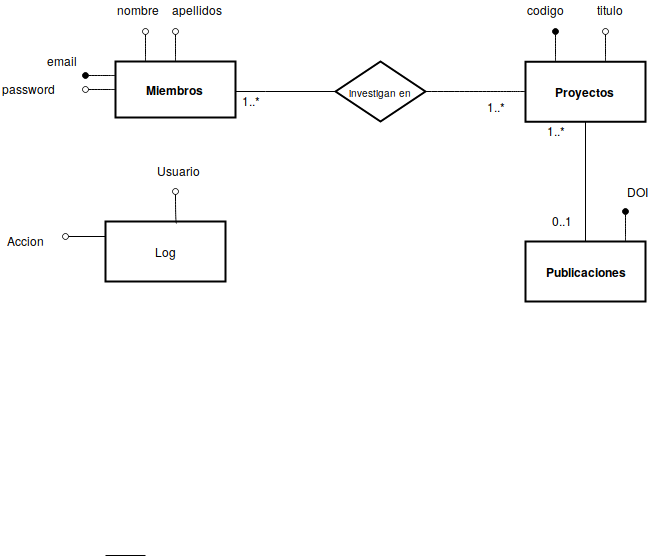
\includegraphics[scale=0.65]{./diagrama_er.png}
\end{figure}

	
\medskip
Las tablas de la base de datos son las siguientes:
\begin{itemize}
	\item MIEMBROS(NOMBRE, APELLIDOS, CATEGORIA, \textbf{EMAIL}, PASSWORD	TELEFONO, URL, DEPARTAMENTO, CENTRO, UNIVERSIDAD, DIRECCION, FOTO, ES\_DIRECTOR, ES\_ADMIN, BLOQUEO, MIEMBRO\_ANTIGUO) 
	\item PROYECTOS(\textbf{CODIGO},TITULO,FECHA\_COMIENZO,FECHA\_FIN,DESCRIPCION,
	ENTIDADES,CUANTIA,\textit{INVESTIGADOR\_PPAL},COLABORADORES,URL)
	\item PUBLICACIONES(\textbf{DOI}, TITULO, AUTORES,FECHA,ABSTRACT, KEYWORDS,URL,\textit{PROYECTO}) 
	\item LOG(USUARIO,FECHA,HORA,ACCION)
\end{itemize}
\section{Aspectos relevantes del desarrollo.}
\subsection{HTML y CSS.}
El aspecto de la aplicación es el siguiente:
\begin{figure}[H]
	
\end{figure}
En cuanto al uso de CSS todas las reglas se encuentran en el archivo \emph{/css/estilos.css}. Para hacer un diseño responsive, se han tenido en cuenta 2 dispositivos: $max-device-width: 480px$ y $(min-device-width: 768px) and (max-device-width: 1024px)$
\subsection{PHP.}
En la carpeta \emph{/php} se encuentran los archivos que realizan los procedimientos PHP. A continuación se detallan dichos archivos:
\begin{itemize}
	\item \textbf{borrar.php}. Realiza las llamadas a los distintos métodos de la BD para borrar miembros,publicaciones o proyectos. Además, se encarga de resolver la integridad de datos poniendo a $NULL$ las referencias externas. 
	\item \textbf{editar.php}. Muestra los formularios de edición.
	\item \textbf{backup.php}. Realiza un backup de la base de datos y guarda las sentencias SQL en un archivo cuyo nombre se forma con la fecha y hora actuales. 
	\item \textbf{restaurarBD.php}. Lee y ejecuta las sentencias SQL del último archivo de backup para restaurar la base de datos. 
	\item \textbf{db.php}. Contiene las funciones que realizan llamadas a la base de datos.
	\item \textbf{nuevoMiembro.php, nuevoProyecto.php, nuevaPublicacion.php.} Obtienen los datos de los formularios correspondientes y realizan una llamada a la base de datos.
	\item \textbf{editarMiembro.php, editarProyecto.php, editarPublicacion.php.} Obtienen los datos de los formularios correspondientes y realizan una llamada a la base de datos.
    \item \textbf{listMiembros.php, listProyectos.php, listPublicaciones.php, listLog.php}. Obtienen los datos almacenados en la base de datos y los listan añadiendo cuando es posible los botones que posibilitan la edición y el borrado.
    \item \textbf{login.php, logout.php}. Gestionan el login en el sistema mediante el uso de sesiones.
    \subsection{JAVASCRIPT.}
    Se ha hecho uso de Javascript para validar los distintos formularios(\emph{/js/validacion.js}), en especial, el formulario
	para registrar un nuevo miembro. En particular, se comprueba que los campos email, nombre, apellidos y contraseña no son vacíos y que las fechas de las publicaciones y proyectos no son vacías(en cuyo caso se indica el formato que debe ser introducido).
	%Paginador
	%\subsection{Otras tecnologías}
\end{itemize}
\end{document}